\documentclass{article}
\usepackage{amsthm}
\usepackage{amssymb}
\usepackage{mathrsfs}
\usepackage{float}
\usepackage{multirow}
\usepackage{verbatim}
\usepackage{fancyhdr}
\usepackage{subfigure}
\usepackage{color}
\usepackage{mathtools}
\usepackage{mathrsfs}
%\usepackage{natbib}
\usepackage{sectsty}
%\usepackage[title]{appendix}
\usepackage{threeparttable}
\usepackage{dcolumn}
\usepackage{booktabs}
\usepackage{indentfirst}
\usepackage{setspace}
\usepackage{bm}
\usepackage{enumerate}
\usepackage{geometry}
\usepackage[UTF8]{ctex}
\usepackage{multicol}
\usepackage{hyperref}
\usepackage{siunitx}			%更好看的物理单位(手打其实更快些)
\usepackage{lmodern}			%一种编码字体
\usepackage{amsmath}			%数学公式扩展
\usepackage[utf8]{inputenc}
\usepackage{ctex} %导入中文包
\usepackage{geometry} %设置页边距的包

\usepackage{pdfpages} %本文最重要的一个包,就是将PDF文件加入到封面位置
%\usepackage[hidelinks]{hyperref}


\usepackage{geometry}%页面设置
\usepackage{graphics}%图片设置
\usepackage{caption}%注释设置

\bibliographystyle{plain}
\geometry{a4paper,scale=0.8}
\title{2022年秋计算物理——Homework1}
\author{中国科学技术大学物理学院2020级\\曾郅琛      PB20071431}
\begin{document}
    \maketitle
    \setlength{\parindent}{2em}
    \maketitle
	\textbf{摘要:}利用C++及Python解决以下问题:用Schrage方法编写随机数子程序,用指定间隔(非连续$l >1$)
    两个随机数作为点的坐标值绘出若干点的平面分布图。再用
    $<x^k>$测试均匀性(取不同量级的N值,讨论偏差与N的关系)、
    $C(l) $测试其2维独立性(总点数$N > 10^7$)	
	
    \textbf{关键字:}Schrage方法;均匀性;独立性

    \section{算法及实现}
        \subsection{16807产生器Schrage方法}
            利用线性同余法:$I_{n+1}=(aI_n+b)$ mod $m,$  $x_n=I_n/m,$ 取$a=16807,b=0,m=2^{31}-1$,
            在此基础上,通过Schrage方法,得到$az$ mod $m$值大小,即可产生不超过计算机32位机的最大数据范围。

            算法实现如下:
\bigotimes 
            \begin{itemize}
                \item 利用教材上1.1.1.4种子值方法生成关于系统时间的种子值$Seed(\;)$函数,作为起始随机数值;
                \item 接着利用生成的种子值,在$Sch \;16807(int \;z)$中可以返回第二个随机数,作为递归子函数;
                \item 之后,通过$Save\;Random(int\;seed,\,int \, N,\,char \,const \,*url)$函数,
                        在生成的种子基础上不断生成随机数$z$,并每次计算$z/(2^{31}-1)$,得到指定数目$N$个$[0,1]$范围内随机数,并存入$*url$文件内。
                \item 最后,将以上函数封装成类$class\; Sch {\;}$,并组织成$main{\;}$函数的库函数。
                \begin{figure}[H]
                    \centering
                    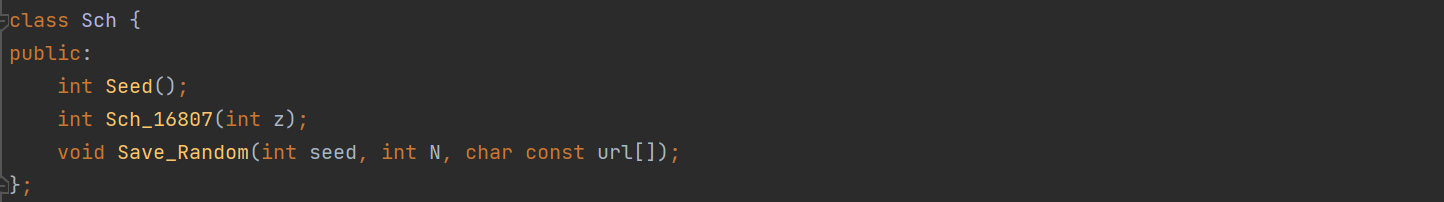
\includegraphics[width= .8\textwidth]{picture/111.png}
                    \caption{类封装函数}
                \end{figure}
            \end{itemize}
        \subsection{均匀性测试检验}
            在均匀性检验过程中读文件按行读取数据,并将读取string转化为double类型:
            \begin{figure}[H]
                \centering
                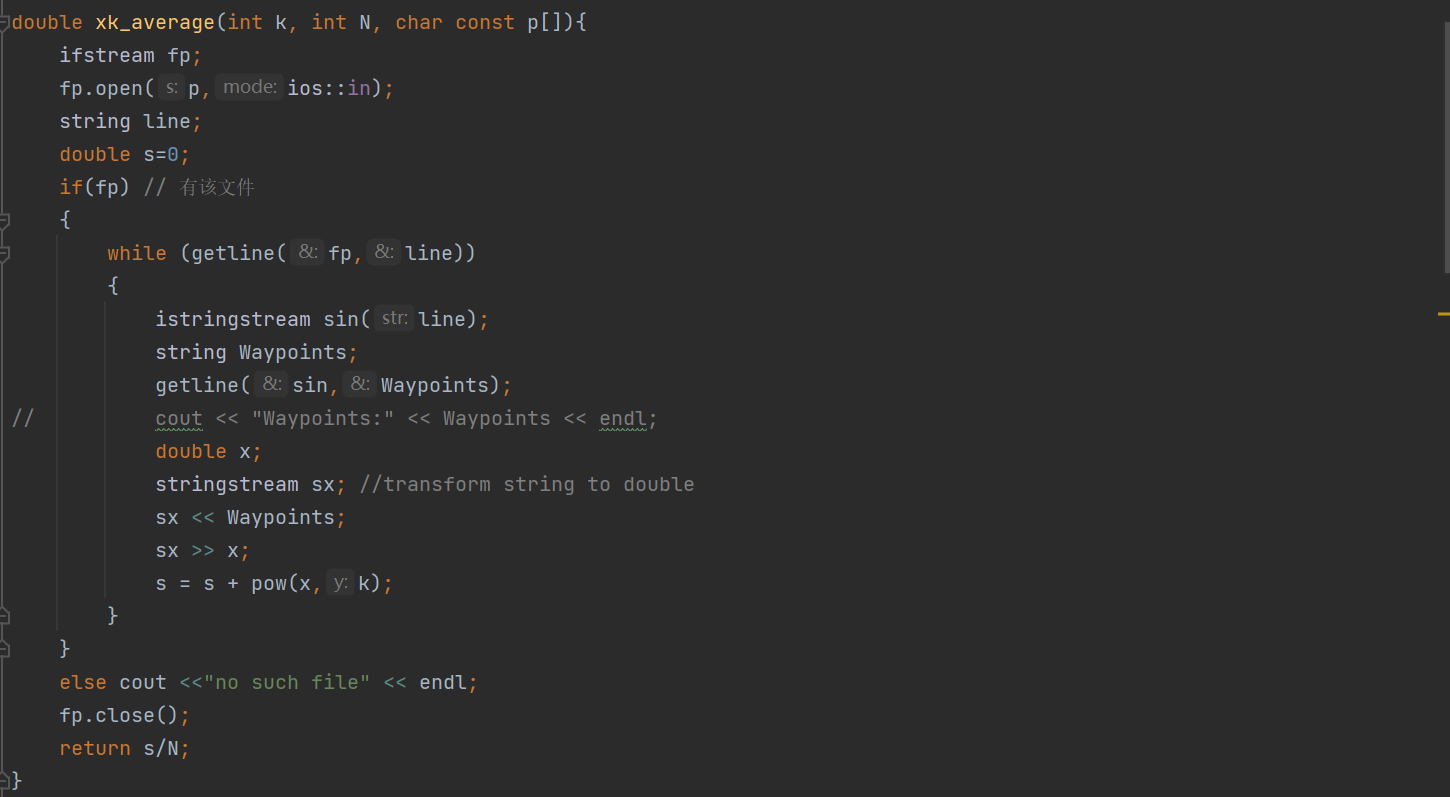
\includegraphics[width= .8\textwidth]{picture/11.png}
                \caption{$<x^k>$计算函数}
            \end{figure}

        \subsection{独立性测试检验}
            由概率论知识,独立性检验标准中间距为$l$的自相关函数$C(l)$:
                $${
                C(l)=<x_{n} x_{n+1}>-<x_n>^2/<x_n^2>-<x_n>^2
                }$$
            
            在$<x^k>$计算函数基础上,只需计算$<x_{n} x_{n+1}>-<x_n>^2$大小,在算法实现中,通过创建一个动态数组,先读出$l$个数据,
            此后的数据在读取时更新动态数组,如此持续下去,最后释放空间,使用动态数组避免占用缓存空间:
            \begin{figure}[H]
                \centering
                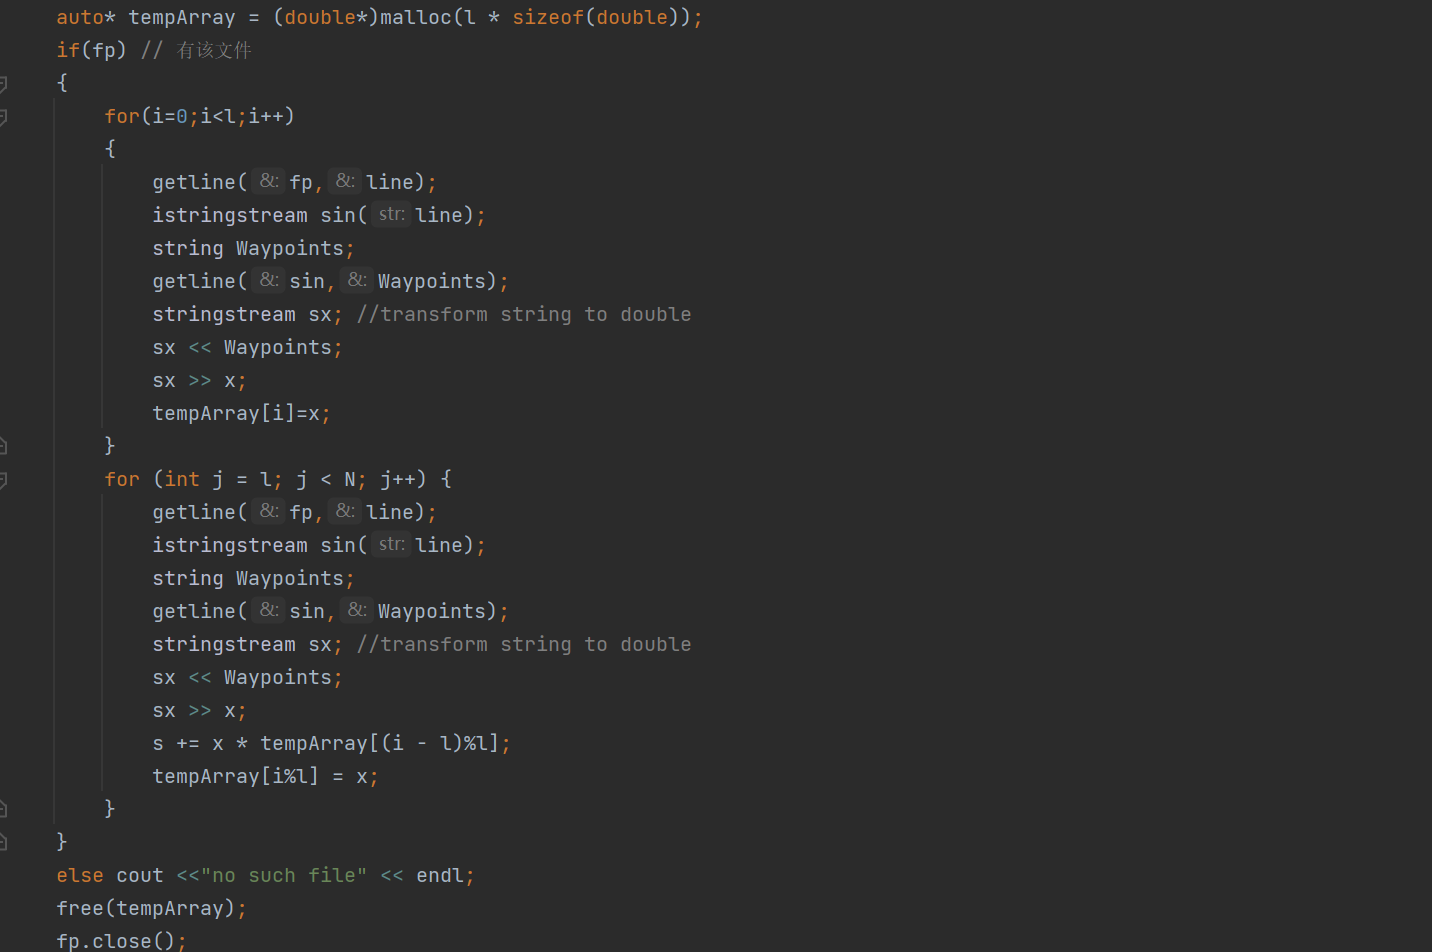
\includegraphics[width= .8\textwidth]{picture/222.png}
                \caption{自相关函数$C(l)$核心代码}
            \end{figure}

            \section{结果分析讨论}
                \subsection{随机数平面分布图}
                用指定间隔(非连续 l >1),本实验取l=4,两个随机数作为点的坐标值绘出若干点的平面分布图。利用python中matplolib库函数作图如下:
                \begin{figure}[H]
                    \centering
                    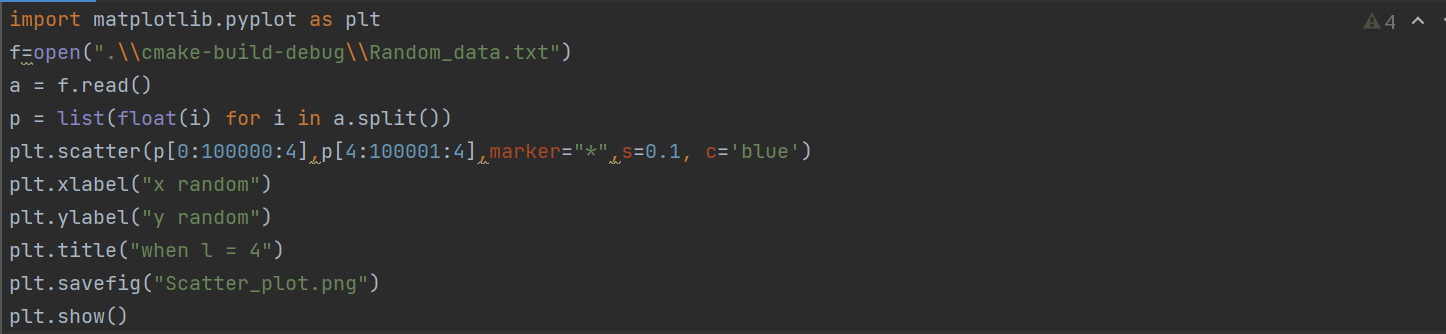
\includegraphics[width= .8\textwidth]{picture/333.png}
                    \caption{随机数分布图代码}
                \end{figure}
                \begin{figure}[H]
                    \centering
                    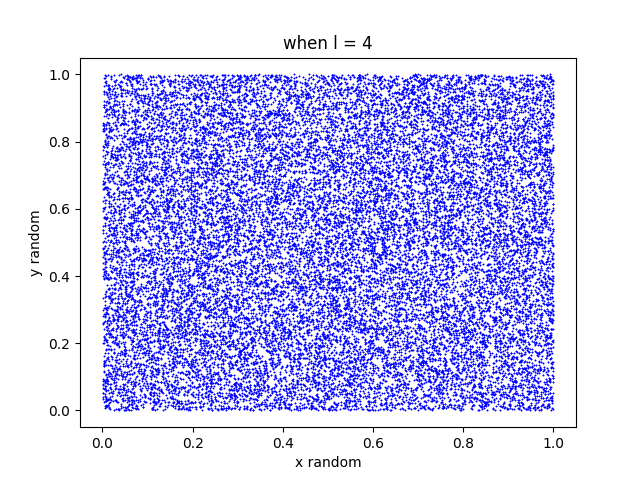
\includegraphics[width= .8\textwidth]{picture/Scatter_plot.png}
                    \caption{随机数二维分布图}
                \end{figure}
                \newpage
                \subsection{均匀性检验结果}
                
                \begin{figure}[htbp]
                    \begin{minipage}[t]{0.3\textwidth}%并排放两张图片,每张占页面的0.5,下同。
                        \centering
                        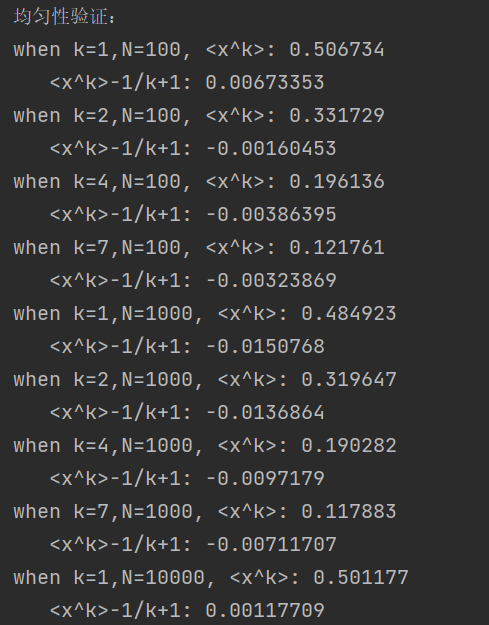
\includegraphics[width=\textwidth]{picture/0.png}
                        \caption{result-1}%注释1.jpg
                        \end{minipage}
                    \begin{minipage}[t]{0.3\textwidth}
                        \centering
                        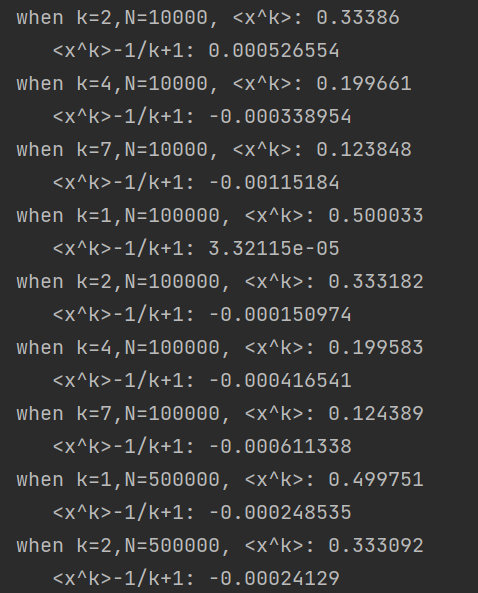
\includegraphics[width=\textwidth]{picture/00.png}
                        \caption{result-2}
                        \end{minipage}
                    \begin{minipage}[t]{0.3\textwidth}
                        \centering
                        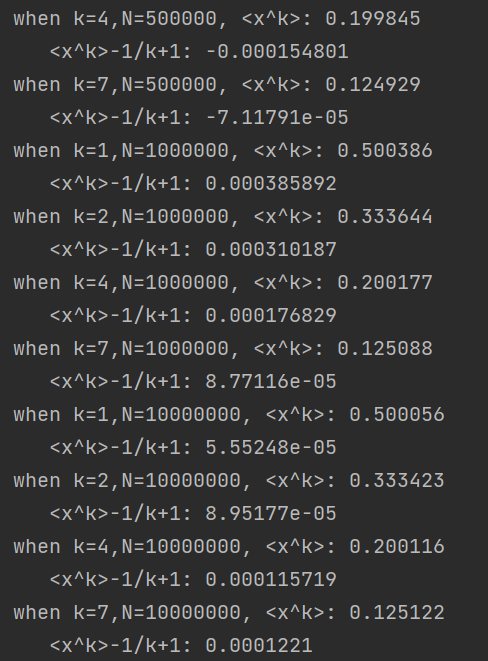
\includegraphics[width=\textwidth]{picture/000.png}
                        \caption{result-3}
                        \end{minipage}
                \end{figure}

                    由结果可以看出:

            
                    \begin{itemize}
                        \item  $<x^k>$与$1/(k+1)$间距在$0.001~0.000001$范围内,差距较小;
                        \item  随着N的增大,$<x^k>$与$1/(k+1)$间距呈现下降趋势;
                        \item  $<x^k>-1/(k+1)$大小与$1/\sqrt{N}$呈现一定的正比关系;    

                    \end{itemize}
                    \begin{figure}[H]
                        \centering
                        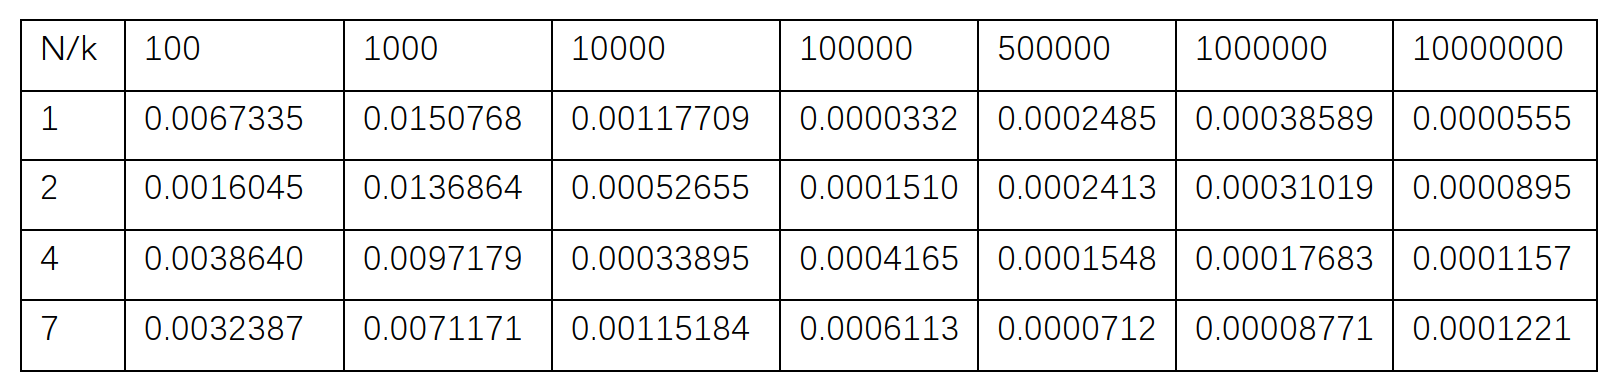
\includegraphics[width= .9\textwidth]{picture/bg.png}
                        \caption{$|<x^k>-1/(k+1)|$与N、k关系}
                    \end{figure}                    
                    \subsection{独立性检验结果}
                    \begin{figure}[H]
                        \centering
                        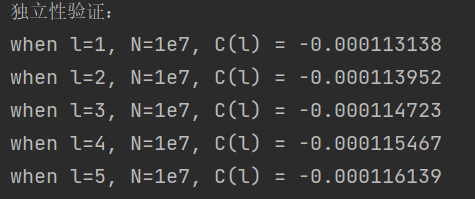
\includegraphics[width= .6\textwidth]{picture/22222.png}
                        \caption{$C(l)$在$N=10^7$结果}
                    \end{figure}
                        理想情况下,$C(l)=0$,在实验中由于随机数的产生并非真随机数,故而存在一定的相关性,
                        所以即使当$N=10^7$时,$C(l)$仍然在0.0001量级,无法做到完全为0。
                    
            \section{总结与心得}
                        在此次实验中自我编写了16807随机数生成器,并通过Schrage方法解决了溢出问题,最后通过取点画图以及均匀性验证,证明了随机数较为均匀;
                        同时也在验证独立性过程中发现该随机数产生并非每个数都是独立的,存在一定的相关性,也间接证明了此方法为伪随机数产生方法。

                        从个人而言,此次实验学会C++编写以及matplotlib画图,进一步提高编程能力,也为后面蒙特卡罗方法奠定基础。
                       
                    \end{document}